% Correcting the title chapter page
\fancypagestyle{plain}{%
    \fancyhf{}
    \fancyhead[RO,LE]{\bfseries \thepage}
    \fancyhead[CO]{\rightmark}
    \fancyhead[CE]{\leftmark}
    \renewcommand{\headrulewidth}{0.4pt}}

\chapter{Simetrije u klasičnoj i kvantnoj mehanici}
\label{ch:klasicna}

U prošlim poglavljima smo izložili teoriju \emph{konačnih} grupa i njihovih reprezentacija.
Teorija kontinuiranih \emph{beskonačnih} grupa ima svojih posebnosti pa kako
bismo olakšali izlaganje i razumijevanje veza s fizikom, prvo ćemo
prodiskutirati neke općenitije aspekte realizacije simetrija u klasičnoj
i kvantnoj mehanici. Očekuje se da čitaoc vlada osnovama kvantne mehanike,
a kratki podsjetnik dan je u dodatku \ref{sec:qm}.


\section{Transformacije i tenzori}
\label{sec:tenzori}

Vidjeli smo upravo u odjeljcima \ref{sec:dipolni} i \ref{sec:degeneracija} kako
simetrije imaju netrivijalne posljedice na moguća makroskopska
svojstva kristala. U tim primjerima sam fizikalni objekt, kristal, je bio
simetričan tj. isti prije i poslije djelovanja transformacije rotacije.
To i jest uobičajeno laičko razumijevanje značenja riječi \emph{simetrija}. Međutim,
mnoge važne realizacije simetrija u prirodi nisu na razini pojedinih
fizikalnih sustava, nego na razini zakona prirode. Na primjer, zakoni mehanike
i gravitacije su simetrični na sve rotacije, ali Sunčev sustav to nije.
Na rotacije su simetrični i zakoni kvantne mehanike, ali pojedini atomi općenito
nisu.
Svejedno, mnoga svojstva Sunčevog sustava i atoma su diktirana simetrijama
zakona koji tim sustavima upravljaju.
U kasnijim poglavljima ćemo na konkretnim primjerima vidjeti kako se simetrije
prirode odražavaju u konkretnim općenito nesimetričnim sustavima, no
sad ćemo najprije uspostaviti relevantnu terminologiju i pomoću nje još
malo produbiti ovu generičku ideju.


\begin{definicija}[invarijantnost i kovarijantnost]
Fizikalna veličina je \emph{invarijantna} na neku transformaciju ako se
pri toj transformaciji ne mijenja.

Jednadžba koja opisuje fizikalni sustav je \emph{kovarijantna}\footnote{%
Pojmovi kovarijantnosti i kontravarijantnosti
komponenata vektora i tenzora koje srećemo u teoriji relativnosti
("gornji" i "donji" indeksi), a zapravo potječu iz diferencijalne 
geometrije nemaju veze s ovom kovarijantnosti.  To su samo homonimi.}
na neku transformaciju ako se pri toj transformaciji 
njen \emph{oblik} ne mijenja.
\end{definicija}


Tako su na primjer masa ili naboj primjeri veličina invarijantnih na rotacije.
S druge strane, Newtonove jednadžbe za sustav dva tijela koja gravitiraju
\begin{eqnarray}
 m_1 \ddot{\vec{r}}_1 & = & G \frac{m_1 m_2}{|\vec{r}_2 - \vec{r}_1|^3}
    (\vec{r}_2 - \vec{r}_1) \label{eq:newton1} \,, \\
 m_2 \ddot{\vec{r}}_2 & = & G \frac{m_1 m_2}{|\vec{r}_1 - \vec{r}_2|^3}
    (\vec{r}_1 - \vec{r}_2) \,,
\end{eqnarray}
su kovarijantne pri rotacijama. Uvjerimo se u to tako da zarotiramo
sustav za neki kut $\theta$ oko osi usmjerene u smjeru jediničnog vektora $\hat{\vec{n}}$.
Pritom se koordinate položaja prvog tijela mijenjaju kao
\begin{align*}
(\vec{r}_{1})_i \to (\vec{r}_{1}')_i &= \sum_j R_{ij}(\hat{\vec{n}},\theta) 
   (\vec{r}_{1})_j \;, \qquad& \text{(zapis po komponentama)}\\
\vec{r}_{1}\to \vec{r}_{1}' &= R(\hat{\vec{n}},\theta) 
   \vec{r}_{1}\;, \qquad& \text{(matrični zapis)}
\end{align*}
i isto za položaj drugog tijela $\vec{r}_2$.
Ovdje je $R(\hat{\vec{n}},\theta)$ standardna matrica rotacije u trodimenzionalnom
prostoru. Na primjer, za rotaciju oko $z$-osi je
\begin{equation}
R(\hat{\vec{z}},\theta) = \begin{pmatrix}
\cos\theta &  -\sin\theta &  0 \\
\sin\theta &  \cos\theta &  0 \\
    0  &       0     &  1 
\end{pmatrix} \;.
\label{eq:matrot}
\end{equation}
Sada iz (\ref{eq:newton1}) slijedi da je nakon transformacije
jednadžba gibanja za npr. $\vec{r}'_1$ 
\begin{equation}
\begin{split}
m_1 \ddot{\vec{r}}'_1 &= m_1 R \ddot{\vec{r}}_1 \\
   &= G \frac{m_1 m_2}{|\vec{r}_2 - \vec{r}_1|^3}
    (R\vec{r}_2 - R\vec{r}_1) \\
   &= G \frac{m_1 m_2}{|\vec{r}_2 - \vec{r}_1|^3}
    (\vec{r}'_2 - \vec{r}'_1) \\
   &= G \frac{m_1 m_2}{|\vec{r}'_2 - \vec{r}'_1|^3}
    (\vec{r}'_2 - \vec{r}'_1) \;,
\end{split}
\label{eq:kovarijantniNewton}
\end{equation}
i isto za $\vec{r}'_2$, gdje smo radi jednostavnosti prestali
pisati argumente matrice rotacije $R = R(\vec{n},\theta)$
i gdje smo u zadnjem redu iskoristili svojstvo da se iznos
vektora pri rotacijama ne mijenja.
Dakle, jednadžbe zarotiranog sustava imaju isti oblik
(kovarijantne su) premda su konkrentne vektorske veličine
u njima različite tj. $\vec{r}'_{1,2} \neq \vec{r}_{1,2}$.
Drugim riječima, zarotirani sustav poštuje iste zakone kao
i originalni. Trećim riječima, nikakvim eksperimentima stanovnici
drugog zarotiranog sustava ne mogu zaključiti da je sustav zarotiran.
Četvrtim riječima, u prirodi su svi smjerovi ekvivalentni.

Ova i daljnja diskusija podrazumijevaju da govorimo o \emph{aktivnim}
transformacijama koje djeluju na sam fizikalni sustav (vidi
str. \pageref{aktivna}). U \emph{pasivnom}
pristupu u kojem transformiramo samo koordinatni sustav,
ovako napisane jednadžbe su \emph{invarijantne} jer
ako $\vec{r}$ i $\vec{F}$ promatramo kao elemente vektorskog prostora,
a ne kao trojke koordinata tih vektora u nekoj bazi, onda rotacija
koordinatnog sustava ne mijenja same vektore i ono sto je onda
\emph{kovarijantno} je zapis tih jednadžbi po komponentama:
\begin{equation}
       m  \ddot{x}_{i} =  F_{i} \;.
\end{equation}

Kod konstrukcije fizikalnih teorija simetrije prirode će se odražavati
u kovarijantnosti jednadžbi gibanja pa je
važno razviti vještinu prepoznavanja jesu li neke jednadžbe
kovarijantne obzirom na neke transformacije ili nisu. Pogledajmo na primjer
Maxwellove jednadžbe klasične elektrodinamike
\begin{align}
    \nabla \cdot \mathbf{E}  &= \frac{\rho}{\varepsilon_0} \,, \label{eq:maxwell1} \\
\nabla \cdot \mathbf{B}  &= 0 \,, \\
\nabla \times \mathbf{E} &= -\frac{\partial \mathbf{B}}{\partial t}  \,,\\
\nabla \times \mathbf{B} &= \mu_0 \left(\mathbf{J} + 
    \varepsilon_0  \frac{\partial \mathbf{E}}{\partial t} \right) \,. \label{eq:maxwell4}
\end{align}
Gledajući matematičku strukturu članova tih jednadžbi vidimo da je ona
\begin{align*}
    \text{skalar} &= \text{skalar} \,, \\
    \text{skalar} &= \text{skalar}  \,,\\
    \text{vektor} &= \text{vektor}  \,,\\
    \text{vektor} &= \text{vektor} + \text{vektor} \,.
\end{align*}
Zapravo je ovdje riječ o skalarnim i vektorskim \emph{poljima}, dakle veličinama
koje imaju neku skalarnu odnosno vektorsku vrijednost u svakoj točki prostora.
To je pogodan primjer jer su kvantnomehaničke valne funkcije
i kvantna polja, što će nam kasnije biti od velikog interesa, isto polja u tom smislu.

Vidimo da su svi članovi svake pojedine gornje jednadžbe istovrsni i sličnim
razmatranjem kao kod
Newtonovih jednadžbi (\ref{eq:kovarijantniNewton}) lako se uvjeriti da
će jednadžbe zarotiranog
sustava biti istog oblika. Dakle Maxwellove jednadžbe su kovarijantne
na rotacije.
Treba uočiti da za ovakvo razmatranje kovarijantnosti jednadžbi pri rotacijama određujuće svojstvo 
vektora nije to što je on opisan trojkom brojeva niti
to što je on element nekog matematičkog vektorskog prostora već je ključno na koji
se način on transformira pri rotacijama. Skalari se transformiraju trivijalno i
zapravo su invarijantni, dok vektore moramo množiti matricom rotacije:

\vspace*{2ex}
\centerline{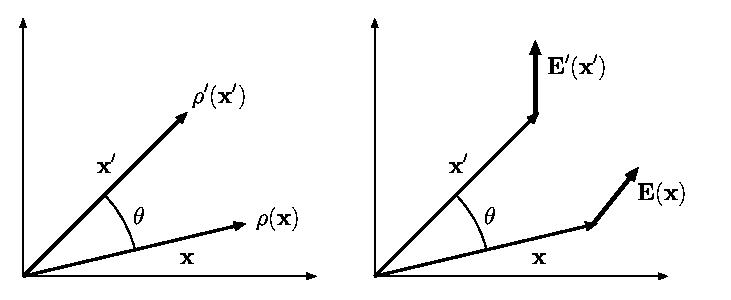
\includegraphics[scale=0.8]{pics/skalarvektor.eps}}

\begin{align*}
    \rho(\vec{r}) &\to \rho'(\vec{r}') = \rho(\vec{r}) \qquad &\textrm{(skalar)} \,, \\
    E_i(\vec{r}) &\to E'_i(\vec{r}') = \sum_j R_{ij}E_j(\vec{r}) 
                 &\textrm{(vektor)} \,,
\end{align*}
gdje je $R_{ij}$ ista matrica (poput (\ref{eq:matrot})) koja rotira
vektor položaja $\vec{r}$. To da se svi vektori rotiraju pomoću identične
matrice je ključno i u ovom kontekstu predstavlja svojevrsnu definiciju
vektora:
\begin{center}
    {vektor} $\equiv$ {objekt koji se pri rotacijama transformira množenjem matricom}
    $R(\hat{\vec{n}}, \theta)$.
\end{center}
Ovo se poopćuje na veličine sa složenijim transformacijskim svojstima,
\emph{tenzore}. 
\begin{definicija}[Tenzor]
\label{def:tenzor}
\emph{Tenzor $n$-tog ranga} (pri rotacijama)  jest veličina $\bbtensor{T}$  koja
se transformira kao
\begin{equation}
 \qquad \bbtensor{T}_{i_1 i_2 \ldots i_n}(\vec{r}) \to \bbtensor{T}'_{i_1 i_2 \ldots i_n}(\vec{r}') =
\sum_{j_1, j_2, \ldots, j_n}
  R_{i_1 j_1}  R_{i_2 j_2} \ldots  R_{i_n j_n} \bbtensor{T}_{j_1 j_2 \ldots j_n}(\vec{r})
 \; . 
\end{equation}
\end{definicija}

Vidimo da su skalari tenzori nultog, a vektori tenzori prvog ranga.
Komponente tenzora drugog ranga $\bbtensor{T}_{ij}$
možemo po želji prikazati matricom.

\begin{primjer}[Tenzor vodljivosti]
U neizotropnom sredstvu (npr. kristalu), smjer struje $\vec{j}$ ne mora biti isti
kao i smjer narinutog električnog polja $\vec{E}$. U tom slučaju Ohmov zakon
glasi
\begin{equation*}
j_i = \sum_j \sigma_{ij} E_j
\end{equation*}
i uključuje tenzor drugog ranga $\sigma_{ij}$ --- tenzor električne vodljivosti.
\end{primjer}

Tenzorsko svojstvo je vezano uz tip transformacije. Tako postoje
npr. \emph{Lorentzovi tenzori} obzirom na Lorentzove tranformacije
(vidi odjeljak \ref{sec:lorentz}), \emph{izotenzori} obzirom na
izospinske transformacije u subnuklearnoj fizici (vidi odjeljak
\ref{sec:izospin}) i drugi.
Kad se tip transformacije ne specificira obično se misli se na rotacije.

\begin{primjer}[Tenzor elektromagnetskog polja]
 Maxwellove jednadžbe (\ref{eq:maxwell1}--\ref{eq:maxwell4}) su očito
 (nekad se kaže \emph{manifestno}) kovarijantne pri rotacijama kako
 je upravo bilo diskutirano. Einsteinu je za razvoj specijalne teorije relativnosti
 bila centralna kovarijantnost tih jednadžbi i pri Lorentzovim
 transformacijama. I premda Maxwellove jednadžbe jesu kovarijantne
 i pri Lorentzovim transformacijama, ta kovarijantnost
 nije manifestna sve dok se sve veličine ne
 zapišu pomoću Lorentzovih tenzora. Tada se gustoća naboja $\rho$ i
 struje $\vec{j}$ ujedinjuju u četverovektor (Lorentzov tenzor prvog
 ranga) $j^{\mu}$, $\mu=0, 1, 2, 3$, dok se električno i magnetsko
 polje ujedinjuju u Lorentzov tenzor drugog ranga
 $F_{\mu\nu}$ kojeg nazivamo tenzor elektromagnetskog polja ili
  ponekad Faradayjev tenzor. Tada jednadžbe (\ref{eq:maxwell1}) i (\ref{eq:maxwell4})
  možemo zapisati u manifestno kovarijantnom obliku
  \begin{equation}
      \partial_{\mu} F^{\mu\nu} = \mu_0 j^{\nu} \;,
      \label{eq:maxwell4D}
  \end{equation}
  što je eksplicitno pokazano u većini modernih udžbenika 
  elektrodinamike poput \cite{Zangwill:2012}.
\end{primjer}

\begin{primjer}[Riemannov tenzor]
Zakrivljenost $n$-dimenzionalnih ploha se standardno opisuje
tzv. Riemannovim tenzorom $R_{abcd}$  (tenzor četvrtog ranga),
gdje je od posebne važnosti za fiziku Riemannov tenzor prostorvremena
koji ima ključnu ulogu u Einsteinovoj općoj teoriji relativnosti.
\end{primjer}


Da bi jednadžba bila kovarijantna svi njeni članovi se moraju transformirati
na isti način. (Kažemo: moraju se transformirati kovarijantno.)
To znači da moraju pripadati istoj reprezentaciji grupe transformacija.
("Pripadati" u smislu da na svakog djeluje ista reprezentacija. Nisu oni
sami reprezentacije!) Tenzori različitih rangova pripadaju različitim
reprezentacijama. Zanimljivo je pitanje, kojim ćemo se baviti
u poglavlju \ref{ch:rotacije}, jesu li te reprezentacije reducibilne.
 
Kakve su posljedice kovarijantnosti jednadžbi gibanja na njihova
rješenja?
Pojedina rješenja sama za sebe naravno nisu invarijantna, ali 
kovarijantnost jednadžbi gibanja implicira da transformacijom rješenja
dobijemo također dobro rješenje.
Na primjer, sustav dva gravitirajuća tijela s reduciranom koordinatom $\vec{r}
= \vec{r}_1 - \vec{r}_2$ ima kao
rješenje jednadžbi gibanja funkciju $\vec{r}(t)$ koja opisuje elipsu.
Sama ta elipsa nije invarijantna na translacije ili rotacije,
međutim, translatirana elipsa $\vec{r}(t)+\vec{a}$ i zarotirana
elipsa $R\vec{r}(t)$ su isto dobra rješenja za bilo koji $\vec{a}$ i $R$
u što se lako uvjerimo uvrštavanjem u Newtonove jednadžbe.
To da translacijom (rotacijom) rješenja također dobijemo rješenje je posljedica
homogenosti (izotropije) prostora.
Provedemo li unatrag ovaj logički sljed vidimo da homogenost
(izotropija) prostora zahtjeva da jednadžbe gibanja budu kovarijantne
obzirom na translacije (rotacije). Konstrukcija fizikalnih teorija se
često svodi na to da identificiramo sve relevantne simetrije i nakon toga
jednadžbe gibanja slažemo od članova kovarijantnih na sve te simetrije\footnote{%
    U tom su smislu posebno moćne tzv. baždarne simetrije koje u
    određenom smislu vode na jednu jedinstvenu jednadžbu gibanja.
To je omogućilo konstrukciju standardnog modela fizike elementarnih čestica
u drugoj polovici XX. stoljeća koji je još uvijek važeća
teorija svih temeljnih prirodnih sila izuzev gravitacije.}.


\begin{primjer}[Vremenska inverzija]
Promotrimo transformaciju inverzije vremena $t \to -t$.
S jedne strane gornje Newtonove jednadžbe su kovarijantne i obzirom na tu vremensku
inverziju, zahvaljujući tome što je diferencijacija po vremenu koja
se tamo javlja uvijek parnog (drugog) reda. 
I stvarno, vremenski invertirano rješenje dvaju gravitirajućih
tijela u gibanju je također dobro rješenje tj. mogući slučaj u prirodi.
No, kao protuprimjer, vremenska inverzija plina koji slobodno izlazi iz plinske boce nije
moguć događaj što ukazuje na to da priroda nije općenito simetrična na vremensku inverziju i
jednadžbe koje opisuju ekspanziju plina ne bi smjele biti kovarijantne
na takvu inverziju. Neka se čitaoc eskplicitno uvjeri u nekovarijantnost drugog
zakona termodinamike na vremensku inverziju i time će dobiti zadovoljavajuće
razumijevanje ove situacije. Stvarno razumijevanje načina na koji je narušena
ova simetrija u zakonima mehanike čestica plina (dakle ne termodinamike) 
predstavlja zloglasni problem strijele vremena \cite{Zeh:2007}.

\end{primjer}

Za potrebe ove knjige definicija \ref{def:tenzor} daje sve što
je potrebno znati o pojmu tenzora. Dodatak \ref{sec:tenzorKaoStroj} daje
jedan drugačiji pogled koji može pomoći u razumijevanju tog
svepristutnog pojma.


\section{Simetrije i zakoni očuvanja}
\label{sec:noether}

U prošlom smo odjeljku promatrali simetrije Newtonovih klasičnih jednadžbi
gibanja. Ispostavlja se međutim da je
Lagrange-Hamiltonova formulacija klasične mehanike znatno pogodnija od
Newtonove za formalizaciju principa simetrije. Naime, centralni objekt
te formulacije je integral lagranžijana tj. akcija
\begin{equation}
S = \int_{t_0}^{t_1}  L\, dt
    \label{eq:akcija}
\end{equation}
koja je invarijantni skalar obzirom na sve simetrije teorije. Razmatranje
je li akcija invarijantna je znantno lakše od razmatranja jesu li jednadžbe
gibanja kovarijantne. Osim toga, u relativističkoj kvantnoj fizici
(kvantnoj teoriji polja), u skladu s načelima relativistike,
vrijeme prestaje imati posebnu ulogu i jednadžbe gibanja
u vremenu se rijetko koriste. 

No, ostanimo još nakratko u svijetu klasične fizike i podsjetimo se da je jedna
od važnih posljedica simetrija u prirodi postojanje očuvanih veličina.
To je posebno lagano vidjeti u Lagrangeovoj formulaciji kako ćemo sada
vidjeti na primjeru simetrija na prostorne translacije.

Prostorne translacije su transformacije oblika
\begin{equation}
\vec{r}\to\vec{r}'=\vec{r}+\delta\vec{r} \,,
\end{equation}
koje čine grupu $(\mathbb{R}^{3},+)$, no grupnoteorijska svojstva nam ovdje
neće biti bitna, do na činjenicu da ona ima beskonačno elemenata parametriziranih
s tri realna broja. Da bi akcija (\ref{eq:akcija}) bila invarijantna potrebno
je da i sam lagranžijan $L$  bude invarijantan\footnote{Strogo uzevši, akcija
    općenito može biti invarijantna i bez da je lagranžijan invarijantan, no to uključuje
    egzotične efekte na rubovima integracije kakvi se ne javljaju u sustavima
    koje ovdje razmatramo.}, odnosno da je promjena lagranžijana
\begin{equation}
 \delta L = L(\vec{r}', \dot{\vec{r}}', t) -  L(\vec{r}, \dot{\vec{r}}, t)
 =0 \,.
\end{equation}
U infinitezimalnom slučaju, ta je promjena
\begin{equation}
    \delta L =  \sum_{i=1}^{3} \frac{\pd L}{\pd r_i} \delta r_i =0 \;,
\end{equation}
iz čega slijedi da je
\begin{equation}
 \frac{\pd L}{\pd r_i}=0 \,, \quad i=1,2,3 \,,
\end{equation}
jer \emph{homogenost prostora} traži da promjena lagranžijana bude nula
za proizvoljan pomak $\delta r_i$.  Kao posljedica toga, lagranžijan
$L(\vec{r},\dot{\vec{r}},t)=L(\dot{\vec{r}},t)$ ne ovisi eksplicitno
o koordinati $\vec{r}$.
Sada Euler-Lagrangeove jednadžbe gibanja,
\begin{equation}
  \frac{\pd L}{\pd r_i}-\frac{d}{d t} \frac{\pd L}{\pd \dot{r}_i}=0 \,,
\end{equation}
daju zakon očuvanja impulsa
\begin{equation}
\frac{d}{d t} \frac{\pd L}{\pd \dot{r}_i}=
\frac{d}{d t} p_i =0  \;,
\end{equation}
odnosno vektor impulsa $\vec{p}$ je konstanta gibanja.

Na sličan način, homogenost vremena znači invarijantnost lagranžijana
na vremenske translacije (jednoparametarska grupa),
što daje zakon očuvanja energije, a izotropija prostora povlači
invarijantnost lagranžijana na prostorne rotacije (troparametarska
grupa) što daje zakon očuvanja momenta impulsa.
Sve ovo gore su samo posebni primjeri sljedećeg općeg teorema.

\begin{teorem}[Noether]
Ako je sustav invarijantan na $n$-parametarsku
grupu transformacija onda postoji $n$ konstanti gibanja.
\end{teorem}

\section{Transformacije kvantnih sustava}

Premda su ideje iz odjeljaka \ref{sec:tenzori} i \ref{sec:noether}
jako prisutne i u kvantnoj teoriji, prikazani formalizam nije sasvim
izravno primjenjiv na kvantne sustave. Za razliku od klasičnih sustava
čije stanje je opisano položajima i impulsima čestica (točkom u faznom
prostoru), kvantni sustavi su reprezentirani kao vektor
u odgovarajućem Hilbertovom vektorskom prostoru, a položaj i impuls
su nekomutirajući operatori na tom prostoru. U dodatku \ref{sec:qm}
su rekapitulirane osnove nerelativističke kvantne mehanike, a
nama je posebno važan Wignerov teorem, po kojem su transformacije simetrije
redovito reprezentirane unitarnim i linearnim opearatorima na
Hilbertovom prostoru stanja\footnote{Druga mogućnost je da operatori
    budu antiunitarni i antilinearni, no odgovarajuće transformacije
    uvijek uključuju inverziju vremena čime se nećemo baviti osim
u odjeljku \ref{sec:tinverzija}.}.
U ovom odjeljku ćemo upoznati neke operatore transformacija kvantnih
sustava, što će nam poslužiti i kao motivacija za općenitije
proučavanje reprezentacija beskonačnih grupa.

\subsection{Kontinuirane prostorne translacije}

Poznato je, vidi odjeljak \ref{sec:qm}, da je konkretno kvantno stanje
$|\alpha\rangle$ moguće prikazati u koordinatnoj bazi kao Schr\"{o}dingerovu
valnu funkciju $\psi_{\alpha}(\vec{r}) = \langle \vec{r} | \alpha\rangle$.
Tako eksplicirana ovisnost o prostornoj koordinati $\vec{r}$ će nam
olakšati razmatranje transformacije translacije u prostoru, a za početak
ćemo uzeti da je prostor jednodimenzionalan, $\vec{r} \to x$.
Zanima nas unitarni operator $U_{r}(a)$ koji djelujući na valnu
funkciju sustava $\psi_{\alpha}(x, t)$ daje valnu funkciju 
\begin{equation}
  \psi'_{\alpha}(x,t)= U_{r}(a)\psi_{\alpha}(x,t) \;,
\end{equation}
tog istog sustava, ali translatiranog za udaljenost $a$. (Kao i uvijek,
smatramo da je transformacija aktivna tj. da djeluje na fizikalni,
a ne koordinatni sustav.)

\centerline{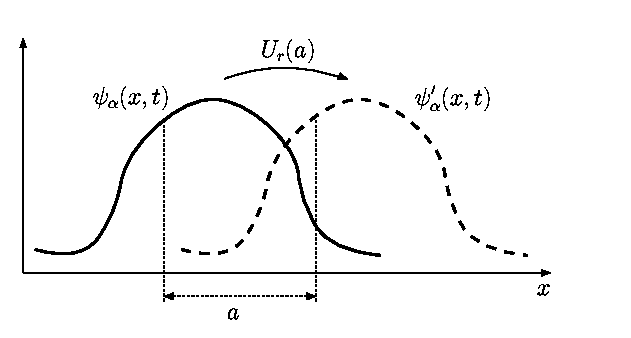
\includegraphics{pics/qmtranslacija.eps}}
Promatrajući crtež, vidimo da vrijedi
\begin{equation}
 \psi'_{\alpha}(x,t)=\psi_{\alpha}(x-a,t) \,,
\end{equation}
odnosno
\begin{equation}
 \psi_{\alpha}(x-a,t)=U_{r}(a)\psi_{\alpha}(x,t)   \,.
 \label{eq:optrans}
\end{equation}
Sada lijevu stranu jednadžbe (\ref{eq:optrans}) razvijemo u Taylorov red
i zbrojimo:
\begin{equation*}
\begin{split}
 \psi_{\alpha}(x-a,t)&=\psi_{\alpha}(x,t)-a\frac{\pd\psi_{\alpha}(x,t)}
{\pd x}+\frac{a^2}{2!}\frac{\pd^2 \psi_{\alpha}(x,t)}{\pd x^2}-\ldots \\
&=\left(1-a\frac{\pd}{\pd x}+\frac{a^2}{2!}\frac{\pd^2}{\pd x^2} - \ldots\right)
\psi_{\alpha}(x,t) \\
&=e^{-a \pd / \pd  x} \psi_{\alpha}(x,t)
\end{split}
\end{equation*}
gdje je eksponencijacija diferencijalnog (ili bilo kakvog drugog) operatora
definirana naznačenom beskonačnom sumom (vidi i dodatak \ref{sec:expmat}).
Usporedbom vidimo da je operator translacije u 1D
\begin{equation}
U_r(a)= e^{-a \pd / \pd  x} \,,
\end{equation}
odnosno, u trodimenzionalnom prostoru ćemo imati
\begin{equation}
U_r(\vec{a})= e^{-\vec{a}\cdot\nabla} \;.
\end{equation}
Poznavajući kvantnomehaničku korespondenciju $-i\hbar\nabla \leftrightarrow
\vec{p}$ imamo konačno općeniti (neovisan o bazi) operator translacije
\begin{equation}
U_r(\vec{a})= e^{-(i/\hbar)\vec{a}\cdot\vec{p}} \;.
\label{eq:Ur}
\end{equation}
Skup translacija čini grupu. Kako svaku translaciju možemo specificirati njenim 
vektorom $\vec{a}$, te kako je kompozicija translacija ekvivalentna zbrajanju
odgovarajućih vektora, vidimo da je ta grupa izomorfna grupi $(\mathbb{R}^3, +)$.

Na malo apstraktniji, ali i općenitiji način, do oblika operatora translacije
možemo doći i razmatranjem koje se ne oslanja na koordinatnu bazu.
Očekivane vrijednosti mjerenja neke veličine koja odgovara hermitskom operatoru $A$
na sustavu u kvantnom stanju $|\alpha\rangle$ 
su dane kao $\langle \alpha | A | \alpha \rangle$ i pri unitarnoj transformaciji $U$
se transformiraju kao 
\begin{equation}
    \langle \alpha | A | \alpha \rangle \to
    \langle U \alpha | A | U \alpha \rangle =
    \langle \alpha | U^{\dagger} A U |  \alpha \rangle =
    \langle \alpha | U^{-1} A U |  \alpha \rangle \;,
\end{equation}
pa transformaciju možemo umjesto na vektorima stanja ekvivalentno promatrati
i na samim operatorima
\begin{equation}
    A \to U^{-1} A U \,.
\end{equation}
Ukoliko nas kao gore zanimaju translacije, očekujemo da se operator položaja
čestice $\vec{x}$ transformira tako da vrijedi
\begin{equation}
    U_{r}(\vec{a})^{-1} \,\vec{x} \, U_{r}(\vec{a}) = \vec{x} + \vec{a} \,.
   \label{eq:defUr}
\end{equation}
Uočite da je plus na desnoj strani ovog izraza konzistentan s definicijom
translacije "udesno" prikazane na gornjoj skici.
Promotrimo sada translaciju za infinitezimalnu udaljenost $\vec{a} \to \vec{\epsilon}$,
$|\vec{\epsilon}| \ll 1$.
Iz razloga kontinuiranosti, odgovarajući operator translacije mora biti
samo infinitezimalno različit od jediničnog operatora pa ga možemo
napisati u obliku
\begin{equation}
    U_{r}(\vec{\epsilon}) = 1 - \frac{i}{\hbar} \vec{p}\cdot\vec{\epsilon} + O(\epsilon^2) \;,
    \label{eq:infinitezimalniUr}
\end{equation}
gdje je $\vec{p}$ operator \emph{definiran} ovim relacijama. Uvrštavanjem
(\ref{eq:infinitezimalniUr}) u (\ref{eq:defUr}) i uspoređivanjem članova
linearnih u $\epsilon_i$ zaključujemo da mora vrijediti
\begin{equation}
    [x_i, p_j] = i\hbar \delta_{ij}\,.
    \label{eq:xpkomutacija}
\end{equation}
Također, kako translacije komutiraju, odgovarajući operatori moraju
zadovoljavati $U_{r}(\vec{\epsilon_1}) U_{r}(\vec{\epsilon_2}) =
U_{r}(\vec{\epsilon_2})U_{r}(\vec{\epsilon_1})$,
pa opet uvrštavanjem i usporedbom članova kvadratnih u $\epsilon_i$
dobivamo
\begin{equation}
    [p_i, p_j] = 0 \;.
    \label{eq:ppkomutacija}
\end{equation}
Ta komutativnost operatora nam sad omogućuje da formalno kompozicijom
operatora N infinitezimalnih translacija za $\vec{\epsilon} = \vec{a}/N$ formiramo 
operator konačne translacije za $\vec{a}$ kao\footnote{Da se uvjerite u ovu
    operatorsku jednakost, uvjerite se da ona vrijedi kad lijeva i desna
    strana djeluju na svojstvene vektore operatora $\vec{p}$, a oni
    čine kompletnu bazu prostora što onda povlači i operatorsku jednakost.}
\begin{equation}
    \lim_{N\to\infty} \left(1 - \frac{i}{\hbar} \frac{\vec{p}\cdot\vec{a}}{N} \right)^N
        = e^{-(i/\hbar)\vec{a}\cdot\vec{p}} \;,
\end{equation}
što je upravo operator translacije $U_r(\vec{a})$ iz (\ref{eq:Ur}).
Naglasimo još jednom da je ovdje operator $\vec{p}$ definiran svojom ulogom
u operatoru translacije (kažemo da on \emph{generira} translacije). 
Kasnije nam daljnja razmatranja trebaju pokazati
da je on kvantnomehanički analogon klasičnom impulsu sustava.


\subsection{Vremenske translacije}

Potpuno analogno translaciji u jednodimenzionalnom prostoru
možemo definirati operator translacije u vremenu $U_{t}(\tau)$
tako da je valna funkcija transformiranog sustava dana kao
\begin{equation}
 \psi'_{\alpha}(x,t) = \psi_{\alpha}(x,t-\tau) = U_{t}(\tau)\psi_{\alpha}(x,t)\,.
\end{equation}
I opet Taylorovim razvojem dobivamo
\begin{equation}
\begin{split}
 \psi_{\alpha}(x,t-\tau)&=\psi_{\alpha}(x,t)-\tau\frac{\pd\psi_{\alpha}(x,t)}
{\pd t}+\ldots \\
&=e^{-\tau \pd / \pd  t} \psi_{\alpha}(x,t) \;,
\end{split}
\end{equation}
te kvantnomehanička korespondencija $i\hbar\pd /\pd t \leftrightarrow H$
daje
\begin{equation}
U_t(\tau)= e^{(i/h)H\tau} \;.
\end{equation}
Ovo vrijedi samo za $H$ konstantan u vremenu, kakav on jest u većini
nama zanimljivih slučajeva (za ostale slučajeve
vidi diskusiju u \cite{Sakurai:2011}, odjeljak 2.1).

Vremenska \emph{translacija} je transformacija koja daje
stanje sustava koji ima isto ponašanje u vremenskom
trenutku $t+\tau$ kao originalni sustav u trenutku $t$. Vremenska
\emph{evolucija} je pak transformacija koja 
daje stanje sustava u trenutku $t+\tau$ djelujući na stanje
tog istog sustava u ranijem trenutku $t$.
Operator vremenske evolucije se može dobiti iz upravo
navedenog, ako primijetimo da je
\begin{equation}
\psi_{\alpha}(x,t-\tau)=e^{(i/h)H\tau}\psi_{\alpha}(x,t)
\end{equation}
pa zamjenom $\tau\equiv t-t'$ imamo 
\begin{equation}
\psi_{\alpha}(x,t')=e^{-(i/h)H(t'-t)}\psi_{\alpha}(x,t)
\end{equation}
Vrijedi dakle
\begin{equation}
U_{\text{evolucija}}(t' -t)=U^{-1}_{\text{translacija}}(t' -t)
=U_{\text{translacija}}(t -t') \;.
\end{equation}

Promotrimo sada operator $A$ takav da je
$[H,A]=0$. Neka je $\psi(x,t)$ svojstveno stanje od $A$ tj.
\begin{equation}
  A\psi(x,t) = a \psi(x,t)
\end{equation}
Tada to isto stanje nakon vremena $(t'-t)$ zadovoljava
\begin{equation}
  A\psi(x,t')= A e^{-(i/h)H(t'-t)} \psi(x,t) =
 e^{-(i/h)H(t'-t)} A \psi(x,t) = a \psi(x,t')
\end{equation}
tj. $A$ je očuvana veličina. Zaključujemo da su
veličine čiji operatori komutiraju s Hamiltonijanom očuvane u vremenu.
Npr. za slobodnu česticu $H=p^2/2m$ i zbog (\ref{eq:ppkomutacija}) imamo
\begin{equation}
   [H,p]=\frac{1}{2m}[p^2,p]=0
\end{equation}
pa je impuls očuvana veličina.



\subsection{Rotacije}

Rotacije u prostoru su transformacije čija nam je važnost
enormna i zbog važnih primjena u fizici kojima je posvećeno
poglavlje \ref{ch:rotacije} i zbog toga što su one paradigmatski
slučaj na kojem se može izložiti većina gradiva teorije kontinuiranih grupa,
kao u poglavlju \ref{ch:lie}.
Konceptualno, unitarni operator $\mathcal{D}(\hat{\vec{n}}, \phi)$
rotacije\footnote{Koristit ćemo
  tradicionalni simbol $\mathcal{D}$ koji dolazi od njemačke
riječi \emph{Drehung} = rotacija.} za kut $\phi$ oko osi $\hat{\vec{n}}$ dobivamo
istim postupkom kao i operatore translacije u prostoru i vremenu,
jedino intrinsična trodimenzionalnost i nekomutativnost rotacija
malo komplicira izvod.

\centerline{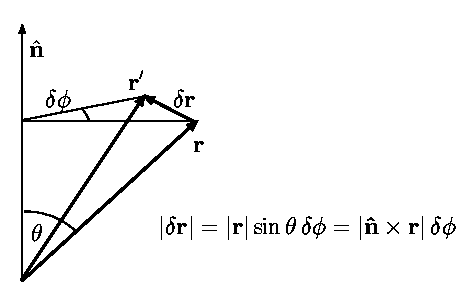
\includegraphics[scale=0.8]{pics/infrotacija.eps}}

Stoga ćemo se odmah usredotočiti na infinitezimalnu rotaciju koja (vidi sliku)
transformira vektor položaja kao
  \begin{equation}
  \vec{r}\to\vec{r}'=\vec{r}+\delta\phi\, \unitn\times\vec{r}  \;.
 \end{equation}
To znači da valna funkcija zarotiranog
sustava treba zadovoljavati
\begin{equation}
\begin{split}
\psi_{\alpha}'(\vec{r}, t)&=\psi_{\alpha}(R(\hat{\vec{n}},\delta \phi)^{-1}
\vec{r}, t) \\
 &=\psi_{\alpha}(\vec{r}-\delta\phi\hat{\vec{n}}\times\vec{r}, t) \\
 &=\psi_{\alpha}(\vec{r}, t)-(\delta\phi\hat{\vec{n}}\times\vec{r})\cdot
  \nabla\psi_{\alpha}(\vec{r}, t) \\
 &= \psi_{\alpha}(\vec{r}, t)-\frac{i}{\hbar}(\delta\phi\hat{\vec{n}}\times
  \vec{r})\cdot \vec{p}\psi_{\alpha}(\vec{r}, t) \\
 &= \left(1-\frac{i}{\hbar}\vec{L}\cdot\hat{\vec{n}}\delta\phi \right)
  \psi_{\alpha}(\vec{r}, t)
\end{split}
\end{equation}

Rotaciju za konačni kut dobijemo kompozicijom N rotacija za $\delta\phi = \phi / N$
gdje $N\to\infty$:

\begin{equation}
\mathcal{D}(\hat{\vec{n}}, \phi)=\lim_{N\to\infty}
\left(1-\frac{i}{\hbar}\vec{L}\cdot\hat{\vec{n}}\delta\phi \right)^N
= e^{-(i/\hbar)\vec{L}\cdot\hat{\vec{n}}\phi}
\label{eq:rotD}
\end{equation}
I opet, ove relacije definiraju operatore $L_i$ kao generatore rotacija,
a kasnija razmatranja pokazuju da je riječ upravo o operatoru koji
odgovara momentu impulsa sustava.
Ukoliko vrijedi $[H,L_{i}]=0$ (a vrijedit će ukoliko neki vanjski utjecaji
ne naruše izotropiju prostora) moment impulsa će biti očuvan.
Poznato je da operatori $L_i$, $i=x,y,z$ zadovoljavaju komutacijske relacije
\begin{equation}
    [L_i, L_j] = i\hbar \epsilon_{ijk}  L_k \,,
    \label{eq:Lkomutacija}
\end{equation}
gdje smo upotrijebili Levi-Civita ili totalno antisimetrični pseudotenzor\footnote{Za
razliku između običnih i pseudotenzora vidi dodatak \ref{sec:aksijalni}.}
trećeg reda definiran
svojim komponentama $\epsilon_{ijk}$ tako da je
\begin{displaymath}
\epsilon_{ijk}=
\begin{cases}
1& \text{ako je $(i,j,k)$ parna permutacija od $(1,2,3)$}, \\
-1& \text{ako je $(i,j,k)$ je neparna permutacija od $(1,2,3)$}, \\
0& \text{inače, tj. ako su dva ili sva tri indeksa ista}.
\end{cases} 
\end{displaymath}
Npr. $\epsilon_{231}=1$, $\epsilon_{213}=-1$, $\epsilon_{221}=0$, itd.

\section{Spin}

U odjeljku \ref{sec:tenzori} vidjeli smo kako veličine u klasičnoj fizici
možemo kategorizirati prema njihovim različitim transformacijskim svojstvima,
recimo na rotacije. Tu smo upoznali tenzore, gdje ovisno o rangu tenzora,
trebamo ga množiti različitim brojem rotacijskih matrica da bismo zapisali
tenzor zarotiranog sustava. Tako očekujemo da i u kvantnoj mehanici jedan
te isti operator
iz (\ref{eq:rotD}) ne može ostvariti
rotaciju proizvoljnog kvantnog sustava.
Uvjerimo se da je to zaista tako
promatrajući rotaciju sustava opisanog vektorskom trojkom valnih funkcija
\begin{equation}
  \vec{\Psi}(\vec{r},t) \equiv (\psi_{x}(\vec{r}, t),
 \psi_{y}(\vec{r}, t), \psi_{z}(\vec{r}, t)) \,.
 \label{eq:psitrojka}
\end{equation}
Takav opis bit će potreban za opis kvantnog stanja čestice za koju nam nije
važan samo njen položaj u prostoru nego i njena orijentacija.
Kao i ranije, tražimo operator $\mathcal{D}(\hat{\vec{n}}, \phi)$, moguće
različit od onog iz (\ref{eq:rotD}), s djelovanjem
\begin{equation}
  \vec{\Psi}'(\vec{r},t) = \mathcal{D}
(\vec{\hat{n}},\phi) \vec{\Psi}(\vec{r},t) \;,
\end{equation}
gdje je $\vec{\Psi}'(\vec{r},t)$ valna funkcija zarotiranog sustava.

\centerline{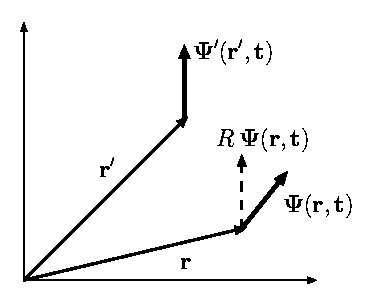
\includegraphics{pics/spin.eps}}

Ukoliko se trojka valnih funkcija iz (\ref{eq:psitrojka}) transformira
pri rotacijama kao standardni vektor, dakle pomoću iste matrice $R(\hat{\vec{n}}, \phi)$
iz odjeljka \ref{sec:tenzori}, iz gornje slike vidimo da zbog promjene
orijentacije čestice treba biti
\begin{gather*}
\vec{\Psi}'(\vec{r}',t)=R \vec{\Psi}(\vec{r},t) \\
\vec{\Psi}'(\vec{r},t)=R \vec{\Psi}(R^{-1}\vec{r},t) 
\end{gather*}
pa imamo, sličnim postupkom kao i ranije
\begin{equation*}
\begin{split}
\mathcal{D}(\vec{\hat{n}},\delta\phi)\vec{\Psi}(\vec{r}, t)&=
 R \vec{\Psi}(R(\hat{\vec{n}},\delta \phi)^{-1}
\vec{r}, t) \\
 &=\vec{\Psi}(R(\hat{\vec{n}}, \delta\phi)^{-1}\vec{r}, t)+
\delta\phi \hat{\vec{n}}\times\vec{\Psi}(
R(\hat{\vec{n}}, \delta\phi)^{-1}\vec{r},t) \\
 &=\vec{\Psi}(\vec{r}-\delta\phi\hat{\vec{n}}\times\vec{r}, t)+
\delta\phi \hat{\vec{n}}\times\vec{\Psi}(\vec{r},t) + O(\delta\phi^2) \\
 &= \vec{\Psi}(\vec{r}, t)-\frac{i}{\hbar}(\delta\phi\hat{\vec{n}}\cdot
  \vec{L})\vec{\Psi}(\vec{r}, t)+
\delta\phi \hat{\vec{n}}\times\vec{\Psi}(\vec{r},t) + O(\delta\phi^2)
\end{split}
\end{equation*}
Vidimo da se obzirom na rotaciju jednokomponentne valne funkcije u prošlom
odjeljku pojavio dodatni član $\delta\phi \hat{\vec{n}}\times\vec{\Psi}(\vec{r},t)$
kojeg ćemo sada zapisati pomoću tripleta matrica $S_{j}$,
definiranih pomoću Levi-Civita pseudotenzora (vidi zadatak \ref{zad:levicivita}):
\begin{equation}
(S_j)_{ik} = i\hbar\epsilon_{ijk} \quad j=1,2,3 \;.
\end{equation}
Konkretno
\begin{align}
S_1& =i\hbar
\begin{pmatrix}
0 & 0 & 0 \\
0 & 0 &-1 \\
0 & 1 & 0
\end{pmatrix} = i\hbar X_1 \,,\\
S_2& = i\hbar
\begin{pmatrix}
0 & 0 & 1 \\
0 & 0 & 0 \\
-1 & 0 & 0
\end{pmatrix} = i\hbar X_2 \,, \\
S_3& = i\hbar
\begin{pmatrix}
0 & -1 & 0 \\
1 & 0 & 0\\
0 & 0 & 0
\end{pmatrix} = i\hbar X_3 \,.
\end{align}
Uz tako definirane matrice imamo
\begin{equation}
\begin{split}
[\hat{\vec{n}}\times\vec{\Psi}]_i &=
\epsilon_{ijk}\hat{n}_j\Psi_k \\
&= -\frac{i}{\hbar}\hat{n}_j (S_j)_{ik}\Psi_k\\
&= -\frac{i}{\hbar}(\hat{\vec{n}}\cdot\vec{S})_{ik}\Psi_k \;,
\end{split}
\end{equation}
što znači
\begin{equation*}
\mathcal{D}(\vec{\hat{n}},\phi)\vec{\Psi}(\vec{r}, t)=
 \left(1-\frac{i}{\hbar}(\vec{L}+\vec{S})\cdot\hat{\vec{n}}\delta\phi \right)
  \Psi(\vec{r}, t) \,,
\end{equation*}
odnosno, operator konačne rotacije ovakvog kvantnog sustava jest
\begin{equation}
\mathcal{D}(\hat{\vec{n}}, \phi)=
 e^{-(i/\hbar)(\vec{L}+\vec{S})\cdot\hat{\vec{n}}\phi} \,.
 \label{eq:rotDJ}
\end{equation}

Hermitske matrice $S_i$ zadovoljavaju iste komutacijske relacije
(\ref{eq:Lkomutacija}) kao i operatori $L_i$ i predstavljaju operatore tzv.
\emph{intrinsičnog}  momenta impulsa poznatog pod nazivom \emph{spin},
za razliku od tzv. \emph{orbitalnog} momenta impulsa kojem odgovaraju
operatori $L_i = (\vec{r}\times\vec{p})_{i}$.
Invarijantnost na rotacije, tj. komutiranje hamiltonijana s operatorom
(\ref{eq:rotDJ}), će onda značiti da je očuvana veličina zapravo
\begin{equation}
\vec{J}=\vec{L}+\vec{S} \,,
\end{equation}
$[H, \vec{J}] = 0$, koju nazivamo \emph{ukupni} moment impulsa, dok je sasvim moguće
da pojedinačno $[H, \vec{L}] \neq 0$ i $[H, \vec{S}] \neq 0$, kao što se na
primjer manifestira u pojavi tzv. vezanja spina i orbite u atomu.
(Elektron usljed orbitiranja "vidi" magnetsko polje
jezgre koje interagira s njegovim magnetskim momentom koji je posljedica
intrinsične vrtnje tj. spina.)

No, ni netom definirani trodimenzionalni operator spina nije najopćenitiji mogući.
U poglavlju \ref{ch:rotacije} vidjet ćemo da ovaj primjer opisuje
vrlo specifičnu situaciju, tzv. česticu spina 1 (točnije $\hbar$),
dok za drugačije iznose intrinsične vrtnje čestica trebamo drugačije
operatore, drugih dimenzionalnosti (npr. spin elektrona koji je iznosa 1/2 
bit će opisan dvodimenzionalnim operatorom).
Za te ćemo potrebe razviti općenitu teoriju
reprezentacija grupe rotacija u kvantnoj mehanici.


\section{Primjena: Blochov teorem}

U ovom ćemo odjeljku pokazati kako primjena teorije grupa elegantno
vodi na važna svojstva valnih funkcija elektrona u kristalu.
\emph{Kristal} je ovdje definiran kao beskonačni trodimenzionalni
sustav atoma koji je invarijantan na translacije 
za bilo koji vektor oblika:
\begin{equation}
  \vec{t}_{\vec{n}} \equiv n_1 \vec{a}_1 + n_2 \vec{a}_2 
  + n_3  \vec{a}_3 \qquad n_{1,2,3}\in\mathbb{Z}\;,
\label{tn}
\end{equation}
gdje su $\vec{a}_{1,2,3}$ tzv. \emph{primitivni vektori} koji definiraju
jediničnu čeliju kristalne rešetke. Prilikom izračuna valne funkcije 
elektronskog
oblaka u kristalu pogodno je zahtijevati da ona zadovoljava tzv.
\emph{Born-von Karmanove periodičke rubne uvjete}:
\begin{equation}
 \psi(\vec{r}) = \psi(\vec{r} + N_1 \vec{a}_1)= \psi(\vec{r} + N_2 \vec{a}_2)
= \psi(\vec{r} + N_3 \vec{a}_3) \;,
\end{equation}
gdje su $N_{1,2,3}$ neki fiksni vrlo veliki ($N_{1,2,3}\gg 1$) prirodni 
brojevi\footnote{
Ovakav zahtjev zamišlja topologiju kristala kao hiper-torusa, što je
dovoljno realistično jer nas ionako topologija ili površinska svojstva
kristala ovdje ne zanimaju, već samo svojstva ``bulk'' materijala poput
specifičnog toplinskog kapaciteta ili električne vodljivosti.
(\emph{Specifični} toplinski kapacitet bakra je naravno isti bez obzira da li je riječ
o ravnoj žici, ploči, beskonačnoj kocki ili pak torusu.)}.

To dalje znači da operatori translacije zadovoljavaju
\begin{equation}
       U_{r}(N_j \vec{a}_j) = U_{r}(0) = 1 \,,  
       \label{eq:Uperiod}
\end{equation}
za svaki $j=1,2,3$ ponaosob (ne sumira se po $j$ u (\ref{eq:Uperiod}),
i odgovarajuća translacijska grupa simetrija ima $N\equiv N_1 N_2 N_3$
elemenata. Kako translacije komutiraju ova grupa je Abelova što
znači da ima $N$ ireducibilnih reprezentacija koje su
sve jednodimenzionalne (cf. npr. Zadatak \ref{zad:1Dabelrep}).
Elementi grupe su generirani translacijom za primitivne vektore
$U_{r}(\vec{a}_j)$  pa tako imamo
\begin{equation}
U_{r}(\vec{a}_1)^{N_1} = 1 
\end{equation}
\begin{equation}
U_{r}(\vec{a}_1) = \exp\Big\{-2\pi i\: \frac{p_1 }{N_1}\Big\} \qquad 
 p_1 \in \{0,1,2,\ldots ,N_1 -1\} \;,
\end{equation}
tj. translacija za $\vec{a}_1$ može biti reprezentirana s
$N_1$ različitih operatora.  Općenita translacija za vektor 
$\vec{t}_{\vec{n}}$ (\ref{tn}) može onda biti reprezentirana jednodimenzionalnim
operatorima oblika
\begin{align}
 U_{r}(\vec{t}_{\vec{n}}) &=
 U_{r}(n_1 \vec{a}_1 + n_2 \vec{a}_2 + n_3  \vec{a}_3) \\
 &= U_{r}(\vec{a}_1)^{n_1} U_{r}(\vec{a}_2)^{n_2} U_{r}(\vec{a}_3)^{n_3} \\
 &= \exp\Big\{ -2\pi i \Big( \frac{n_1 p_1}{N_1} + \frac{n_2 p_2}{N_2} 
 + \frac{n_3 p_3}{N_3} \Big)\Big\} \;,
\label{blochirreps}
\end{align}
tj. s $N$ različitih operatora kako i očekujemo za grupu s $N$ IRREPsa.
Svaka od tih IRREPsa se onda može označiti ("labelirati") s trojkom brojeva $(p_1, p_2, p_3)$
gdje svaki od brojeva $p_j$ može poprimiti bilo koju vrijednost iz
skupa $\{0, 1, 2, \ldots ,N_j -1\}$.
Operator translacije $U_{r}(\vec{t}_{\vec{n}})$ je u konkretnom IRREPsu 
 $(p_1, p_2, p_3)$ reprezentiran operatorom/brojem (\ref{blochirreps}).

Umjesto trojke $(p_1, p_2, p_3)$ za označavanje IRREPsa se obično
upotrebljavaju vektori $\vec{k}$ definirani na slijedeći način. Prvo
definiramo tzv. vektore \emph{recipročne rešetke} $\vec{b}_1, \vec{b}_2,
\vec{b}_3$ putem zahtjeva:
\begin{equation}
   \vec{a}_i\cdot \vec{b}_j = 2 \pi \delta_{ij} \qquad i,j = 1, 2, 3 \;.
\label{defb}
\end{equation}
Sada vektor $\vec{k}$ koji odgovara IRREPsu
$(p_1, p_2, p_3)$ definiramo kao
\begin{equation}
  \vec{k} \equiv \frac{p_1}{N_1}\vec{b}_1 + \frac{p_2}{N_2}\vec{b}_2 + 
  \frac{p_3}{N_3}\vec{b}_3 \;.
\label{defk}
\end{equation}
Iz (\ref{defk}), (\ref{defb}) i (\ref{blochirreps}) slijedi da je
operator translacije za $\vec{t}_{\vec{n}}$ u IRREPsu $\vec{k}$
dan s
\begin{equation}
 U_{r}^{(\vec{k})} (\vec{t}_{\vec{n}}) = 
 e^{-i \vec{k}\cdot \vec{t}_{\vec{n}}} \;,
\end{equation}
i odsad $N$ različitih $\vec{k}$-ova (\ref{defk}) labelira IRREPse.
Vidimo da dimenzija $\vec{k}$ odgovara valnom broju, tj. impulsu
podijeljenom s Planckovom konstantom.

Djelovanje ovih operatora translacije na valne funkcije u datom
IRREPsu mora biti kao i kod svih operatora translacije (\ref{eq:optrans})
\begin{equation}
 e^{-i \vec{k}\cdot \vec{t}_{\vec{n}}} \psi_{\vec{k}}(\vec{r}) =
\psi_{\vec{k}}(\vec{r} - \vec{t}_{\vec{n}}) \;.
\label{bloch}
\end{equation}
Kako je riječ o običnim brojevima (a ne recimo o diferencijalnim
operatorima) dobili smo razmjerno jednostavan uvjet koji valne funkcije
u kristalu moraju zadovoljavati da bi bile svojstvene funkcije operatora
translacije. Takve funkcije se nazivaju \emph{Blochove funkcije}, a
$\vec{k}$ je Blochov valni vektor.
Zašto su one zanimljive?

Kao prvo, ako ih (bez gubitka općenitosti) zapišemo u obliku
\begin{equation}
 \psi_{\vec{k}}(\vec{r}) = e^{+i \vec{k}\cdot \vec{r}} u_{\vec{k}}(\vec{r})
\end{equation}
onda odmah iz (\ref{bloch}) dobijemo uvjet 
\begin{equation}
  u_{\vec{k}}(\vec{r}) = u_{\vec{k}}(\vec{r} - \vec{t}_{\vec{n}})  \;,
\end{equation}
dakle Blochove funkcije su oblika 
$e^{+i \vec{k}\cdot \vec{r}} u_{\vec{k}}(\vec{r})$,
gdje je $u_{\vec{k}}(\vec{r})$ periodička funkcija na rešetci.
S druge strane, operator translacije na rešetci komutira s Hamiltonijanom
\begin{equation}
    [H, U_{r}^{(\vec{k})} (\vec{t}_{\vec{n}}) ] = 0 \;,
\end{equation}
kako i očekujemo od operatora simetrije.
Komutiranje s kinetičkim dijelom je trivijalno jer su i kinetički dio
hamiltonijana i operator translacije funkcije samo impulsa koji
komutiraju međusobno.  Komutiranje s potencijalom je manje trivijalno
i posljedica je periodičnosti $V(\vec{r}) = 
V(\vec{r}+\vec{t}_{\vec{n}})$\footnote{Po analogiji s
    (\ref{eq:defUr}) za svaki operator $A(\vec{r})$ vrijedi
    $U_{r}^{-1}(\vec{t}_{\vec{n}})
A(\vec{r}) U_{r}(\vec{t}_{\vec{n}}) = A(\vec{r}+\vec{t}_{\vec{n}})$,
pa onda to vrijedi i za $A=V$ pa iz toga i iz periodičnosti $V$ odmah slijedi tražena
komutativnost.}.
Posljedica komutiranja dvaju operatora je da oni imaju zajedničke
svojstvene funkcije. To onda povlači
\begin{teorem}[Bloch]
Valne funkcije periodičke rešetke mogu se izabrati kao Blochove funkcije.
\end{teorem}

Ovo onda olakšava rješavanje Schr\"{o}dingerove jednadžbe
za rešetku jer je potrebno naći samo funkcije $u_{\vec{k}}(\vec{r})$ za
svaki $\vec{k}$,
a njihova periodičnost umnogome pojednostavljuje taj zadatak,
kako svjedoče brojni primjeri iz fizike čvrstog stanja.
Blochov teorem se obično izvodi i u udžbenicima fizike čvrstog
stanja, no ovdje smo dali naglasak
na grupno-teorijski pristup tj. korespondenciju s reprezentacijama
grupe translacija.

\subsection*{Zadaci}

\begin{enumerate}[label=\arabic{chapter}.\arabic*.]

\item \label{zad:kronecker} Kroneckerov simbol $\delta_{ij}$, $i,j \in \{1, 2, 3\}$ je tenzor drugog ranga
    obzirom na rotacije. Tenzori su općenito definirani kao veličine 
    \emph{kovarijantne} pri datim transformacijama. Pokažite da je $\delta_{ij}$
    također i \emph{invarijantan}.
\item Pokažite da je operator translacije kvantnomehaničkog stanja,
 $U_{r}(\vec{a}) = \exp \{-\frac{i}{\hbar} \vec{p}\cdot \vec{a} \}$
unitaran. Razmotrite situaciju u koordinatnoj reprezentaciji gdje
je $\vec{p} = -i \hbar \nabla$. Zašto ovaj $i$ ne kvari unitarnost?

\item Neka $\psi(\vec{r}, t)$ zadovoljava Schr\"{o}dingerovu jednadžbu.
Pokažite da će prostorno translatirana $\psi(\vec{r}, t)' = 
U_{r}(\vec{a}) \psi(\vec{r}, t)$ također zadovoljavati Schr\"{o}dingerovu
jednadžbu ako i samo ako je $[H, \vec{p}] = 0$

\item Koristeći fundamentalne kvantnomehaničke komutatore
\begin{equation}
 [x_i, p_j] = i\hbar \delta_{ij}\;, \qquad
 [x_i, x_j] = [p_i, p_j] = 0 \;,
\end{equation}
te svojstva Levi-Civita tenzora, izračunajte komutacijske
relacije angularnog momenta $[L_i, L_j]$.

\item Pokažite da operatori spina $S_i$ također zadovoljavaju komutacijske
relacije angularnog momenta.

\item Pokažite da je $[\vec{J}^2, J_i] = 0$.
\item \label{zad:levicivita} Uvjerite se da se pomoću Levi-Civita tenzora mogu elegantno zapisati
    vektorski produkt i determinanta matrice: $\epsilon_{ijk}a_{j}b_{k}
    = (\vec{a}\times\vec{b})_{i}$, $\epsilon_{ijk}A_{il}A_{jm}A_{kn} = \det A \: \epsilon_{lmn}$.
\end{enumerate}
